\newpage
\subsection{Implementing check}
\visHeader
\hypertarget{checkCard vis}{}

\begin{itemize}

\item[$\blacktriangleright$] Since you're nearly a SDM wizard already, try using concepts we have already learnt to create the control flow for
\texttt{Partition::check} as depicted in Fig.~\ref{fig:sdm_check_start}.

\begin{figure}[htbp]
\begin{center}
  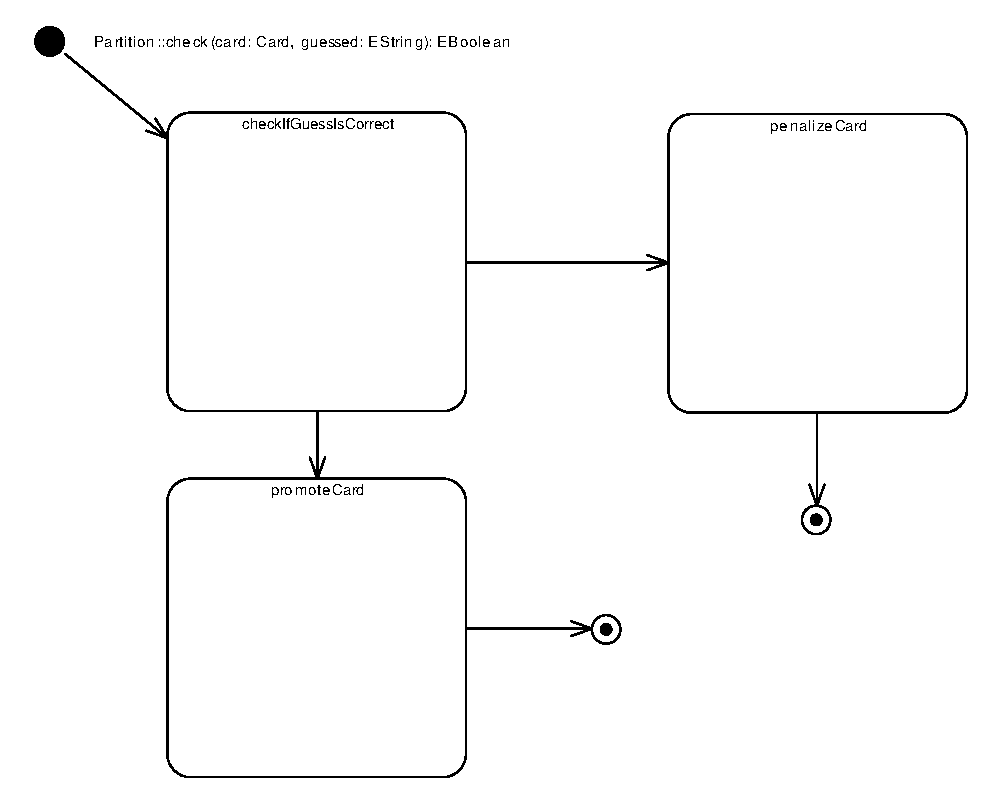
\includegraphics[width=1\textwidth]{ea_activityCheck.pdf}
  \caption{Activity diagram for \texttt{Partition::check}}
  \label{fig:sdm_check_start}
\end{center}
\end{figure}

\item[$\blacktriangleright$] To check if the guess was correct, create an object variable that is bound to the argument \texttt{card}. This will
represent the card the user picked from the learning box. Remember that this binding is implicitly defined by choosing the name of the argument as the
name of the object variable (Fig.~\ref{fig:sdm_check_addCard}).

\begin{figure}[htbp]
\begin{center}
  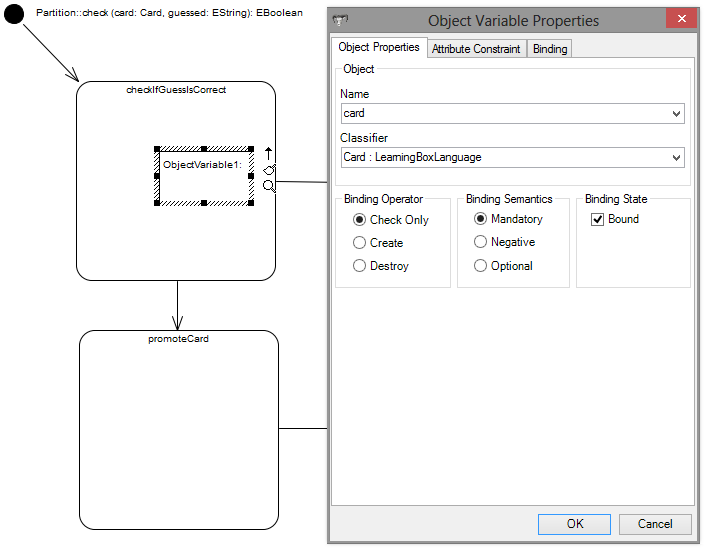
\includegraphics[width=0.7\textwidth]{ea_addCheckCard}
  \caption{Add the card to be checked}
  \label{fig:sdm_check_addCard}
\end{center}
\end{figure}

% Will this attribute constraint also be defined for textual??
\item[$\blacktriangleright$] Now that we have the card to be checked, we need to compare the user's guess to the actual answer on the
back of the card. To do this we need to specify an \emph{Attribute Constraint}. Choose the \texttt{Attribute Constraint} tab as depicted in
Fig.~\ref{fig:sdm_check_att_constraint} ({\bf get this image}). In this dialogue, choose the attribute to be used in formulating the constraint
(\texttt{back})({\bf you sure it's not face?}), and the type of \texttt{Expression} used to express it. As we shall compare the back of the card with the user's
guess (passed in as a parameter), we'll need to use a \texttt{ParameterExpression} again to refer to this value.

\item[$\blacktriangleright$] In the previous section, we used a \emph{ParameterExpression} to specify the return value in a stop node. Now, choose the parameter
(\texttt{guessed}), and the type of constraint or \emph{operation} to be executed. In this case, it's an equality check (\texttt{==}). Press the button labelled
\texttt{Add} and admire your first attribute constraint (Fig.~\ref{fig:sdm_check_att_constraint}) ({\bf get this image}).

% Update this screenshot
\begin{figure}[htbp]
\begin{center}
  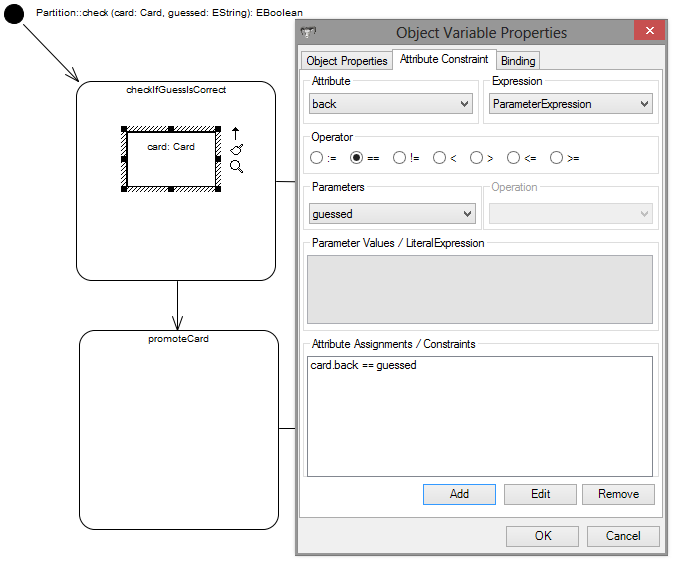
\includegraphics[width=0.8\textwidth]{ea_addAttributeConstraint}
  \caption{Add an attribute constraint with a parameter expression {\bf UPDATE}}
  \label{fig:sdm_check_att_constraint }
\end{center}
\end{figure}

\begin{figure}[htbp]
\begin{center}
  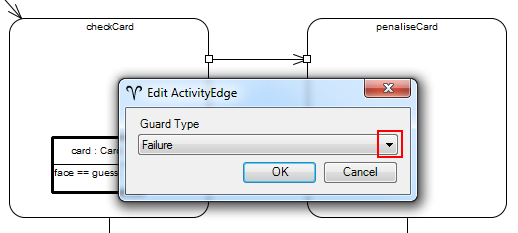
\includegraphics[width=0.75\textwidth]{ea_addTransitionGuard}
  \caption{Add a transition with a guard}
  \label{fig:sdm_check_guard}
\end{center}
\end{figure}

Let's return to the control flow. We now need to explicitly specify how the card is to be moved based on the result of the guess. Such an if/else construct is
built in SDMs via \emph{Edge Guards}.

\item[$\blacktriangleright$] To add a guard to the edge leading from \texttt{Check\-If\-Guess\-Is\-Correct} to \texttt{penalize\-Card}, double click the edge
and set the \emph{Guard Type} in the dialogue (Fig.~\ref{fig:sdm_check_guard}).

\item[$\blacktriangleright$] Choose \texttt{Failure}, and repeat the process for the edge leading to \texttt{promoteCard} by selecting \texttt{Success}.

The next feature of EA and eMoflon that we shall learn about is a means of coping with large patterns\footnote{You thought I was going to say `coping with our
coffee addiction', weren't you?}. It might be nice to visualise \emph{small} story patterns directly in their story nodes, but for large patterns or complex
surrounding control flow, such diagrams would get extremely cumbersome and unwieldy very quickly!  This is indeed a popular argument against visual languages and
it might already have crossed your mind (``this is cute, but it'll \emph{never} scale!''). With the right tools and concepts however, even huge diagrams can be
mastered. We support \emph{extracting} story patterns to their own diagrams, and recommend this in most cases (unless the pattern is really concise and only
contains 2 or 3 object variables).

\item[$\blacktriangleright$] To extract an empty or already partially modelled story pattern, just double-click the corresponding story node
(\texttt{promoteCard}) and choose \texttt{Extract Story Pattern} (Fig.~\ref{fig:sdm_check_extract_storypattern}). Note the new diagram that is immediately
opened and created in the project browser (Fig.~\ref{fig:sdm_new_sub_diagram}).

\begin{figure}[htbp]
\begin{center}
  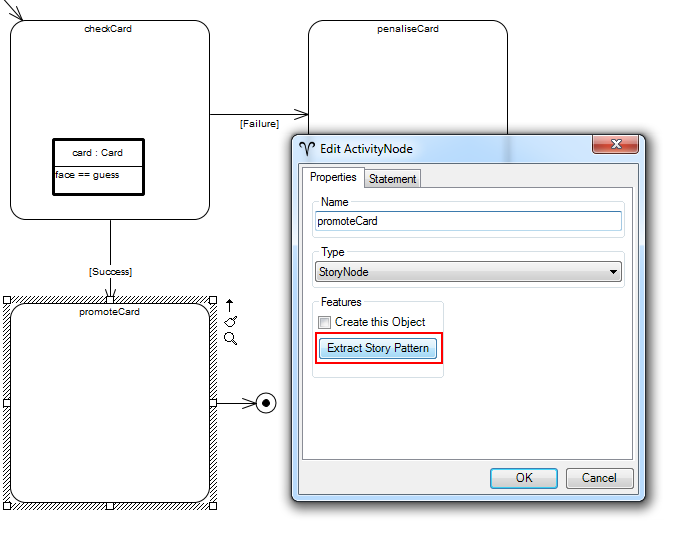
\includegraphics[width=0.75\textwidth]{ea_extractStoryPattern}
  \caption{Extract a story pattern for more space and a better overview}
  \label{fig:sdm_check_extract_storypattern}
\end{center}
\end{figure}

\begin{figure}[htbp]
\begin{center}
  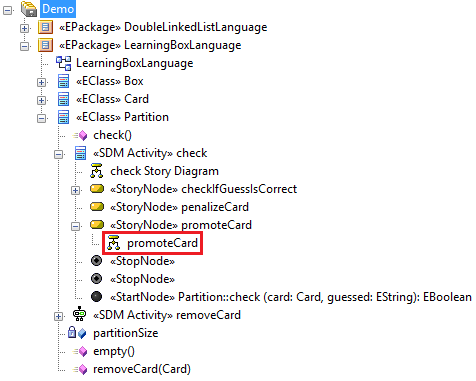
\includegraphics[width=0.75\textwidth]{sdm_new_storypattern_diagram}
  \caption{A new sub diagram is created automatically}
  \label{fig:sdm_new_sub_diagram}
\end{center}
\end{figure}

\item[$\blacktriangleright$] Another EA gesture you should take advantage of is a good ol' \emph{Drag and Drop} action from the project
browser\footnote{Remember the other two gestures we have learnt: Quick Link and Quick Create.}. We can use this as an alternative to the SDM toolbox. To create
an object variable, simply drag and drop the class \texttt{Card} from the project browser and into the extracted story pattern diagram
(Fig.~\ref{fig:sdm_check_bound_card}).

% UPDATE THIS SCREENSHOT
\begin{figure}[htbp]
\begin{center}
  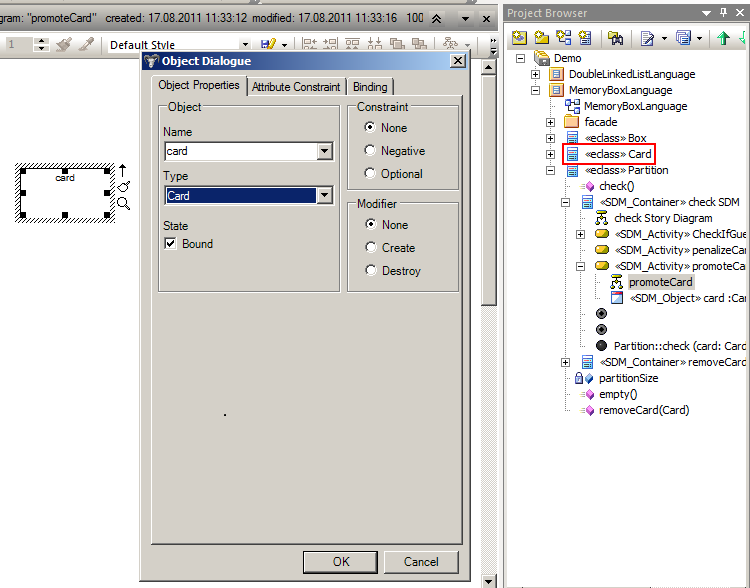
\includegraphics[width=\textwidth]{sdm22RAW}
  \caption{Add an object variable per drag and drop {\bf UPDATE}}
  \label{fig:sdm_check_bound_card}
\end{center}
\end{figure}

A dialogue should pop-up asking if you want to (1) create a simple link (referring to \texttt{Card} as a class), (2) create an Object (as an instance of
\texttt{Card}), or (3) if you want to create a subclass. In our case we want to create an object(variable) and so (2) is the best choice. Since this
\texttt{Paste Element} dialogue is a bit annoying, EA allows you to choose a default for \emph{all} drag and drop gestures.

\item[$\blacktriangleright$] Go ahead and check \texttt{All Drag and Drop} so option (2) is used next time by default. You should also check \texttt{Only show
this dialog when Ctrl+Mouse drag is used}, so that the default is used \emph{without} popping up a confirmation dialogue. Don't worry, if you ever need options
(1) and (3), you  just need to hold \texttt{Ctrl} when dragging to invoke the dialogue and change the settings.

\item[$\blacktriangleright$] After creating the object, you will be asked to set the object variable properties. Set its \texttt{Name} to ``card'' and its
\texttt{Binding State} to ''Bound'' (Fig.~\ref{fig:sdm_new_card_properties}).

\begin{figure}[htbp]
\begin{center}
  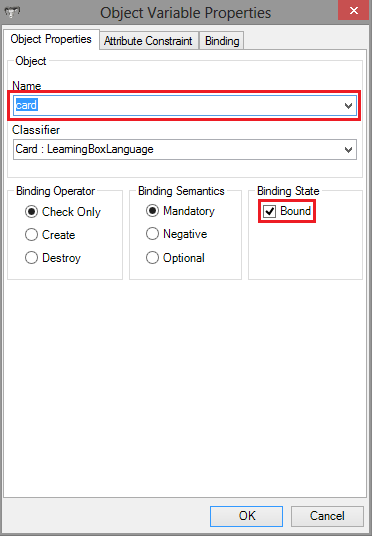
\includegraphics[width=0.5\textwidth]{ea_addBoundCard}
  \caption{Object variable properties of the new card}
  \label{fig:sdm_new_card_properties}
\end{center}
\end{figure}

The main advantage of drag and drop is that the \texttt{Object Variable Pro\-per\-ties} dialogue that pops-up should have the type of the object variable
pre-configured. Choosing the type in the project browser and dragging it in is (for most people) a more natural gesture than choosing the type from a long
drop-down menu. It can really be a great time saver for large metamodels\footnote{Drag and drop is also possible in embedded story patterns (still visualised in
their story nodes).  You must ensure however, that the object variable is \emph{completely} contained inside the story node and does not stick out over any
edge}.

\item[$\blacktriangleright$] Let's move on with the current pattern. Remember that we want to promote the card. As a first step, drag and drop two further
object variables for \texttt{this} (the current partition), and the \texttt{nextPartition}, as depicted in Fig.~\ref{fig:sdm_check_complete_sp}. 

\begin{figure}[htbp]
\begin{center}
  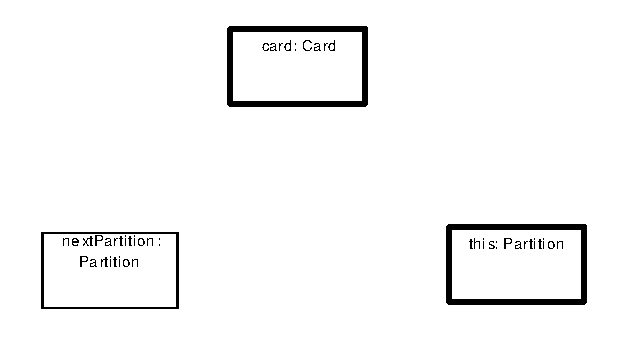
\includegraphics[width=0.8\textwidth]{ea_objVarsCheck.pdf}
  \caption{All object variables for story pattern \texttt{promoteCard}}
  \label{fig:sdm_check_complete_sp}
\end{center}
\end{figure}

An important point to note here is that \texttt{this} and \texttt{card} are visually differentiated from \texttt{nextPartition} by their bold border lines.
This is how we differentiate \emph{bound} \note{Bound vs. Unbound} variables (\texttt{this, card}) from \emph{unbound} or \emph{free} variables like
\texttt{nextPartition}. We already know that matches for bound variables are completely determined by the current context. On the other hand, matches for
unbound variables, have to be determined by the pattern matcher. Such matches are ``found'' by navigating and searching the current model for possible matches
that satisfy all specified constraints (e.g. type of the variable, links connecting it to other variables and attribute constraints). In our case, the next
partition has to be determined by navigating from \texttt{this} via the \texttt{next} link in the metamodel.  

\item[$\blacktriangleright$] Make sure the bound checkbox for \texttt{nextPartition} is left empty, and quick link from \texttt{this} to \texttt{nextPartition}
(or vice-versa) to create a \texttt{next} link variable, as shown in Fig.~\ref{fig:sdm_check_link_variable}.

\begin{figure}[htbp]
\begin{center}
  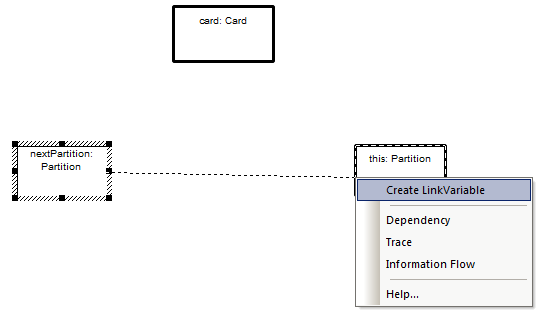
\includegraphics[width=0.85\textwidth]{ea_addLinkVar}
  \caption{Create a link variable.}
  \label{fig:sdm_check_link_variable}
\end{center}
\end{figure}

\item[$\blacktriangleright$] If you've done everything right, your story pattern should now closely resemble Fig.~\ref{fig:sdm_check_complete_activity_node}. 
Reflect on what the pattern expresses.

\begin{figure}[htbp]
\begin{center}
  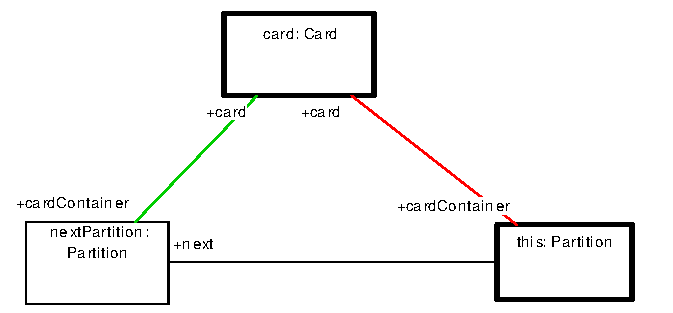
\includegraphics[width=0.8\textwidth]{ea_completeActivityPromote.pdf}
  \caption{Complete story pattern for activity node \texttt{promoteCard}}
  \label{fig:sdm_check_complete_activity_node}
\end{center}
\end{figure}

\item[$\blacktriangleright$] Now repeat the entire process for the story node \texttt{penalizeCard}: extract the story pattern, and create all variables as
depicted in Fig.~\ref{fig:sdm_check_complete_penalize}.  This pattern is quite similar to \texttt{promoteCard}, except it moves the card from \texttt{this} to
\texttt{previous} instead of to \texttt{next}. Exactly the same as before, \texttt{previousPartition} is unbound and must be determined by navigating from \texttt{this}
along the link \texttt{previous}.

\begin{figure}[htbp]
\begin{center}
  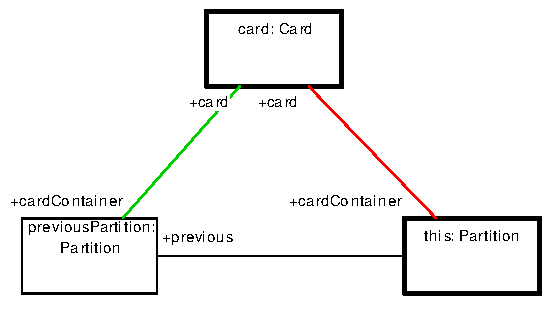
\includegraphics[width=0.8\textwidth]{ea_completeActivityPenalize.pdf}
  \caption{Story pattern for activity node \texttt{penalizeCard}}
  \label{fig:sdm_check_complete_penalize}
\end{center}
\end{figure}

\item[$\blacktriangleright$] To complete our SDM, we need to signalise as a return value if the guess was correct or not (and consequently if the card was promoted or penalised).  To do
\note{Literal-\\ Expression} this, double-click the stop node after \texttt{promoteCard} and choose \texttt{LiteralExpression} as the type of expression
(Fig.~\ref{fig:sdm_check_literal_exp}).

\begin{figure}[htbp]
\begin{center}
  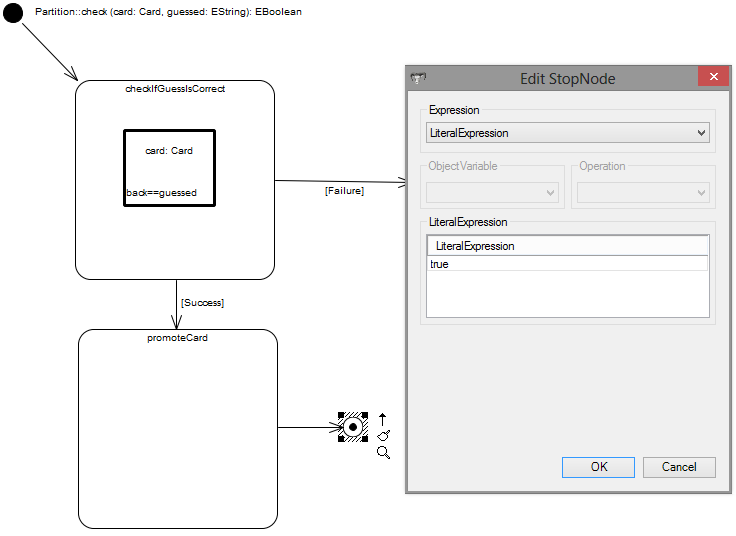
\includegraphics[width=0.6\textwidth]{ea_addStopReturn}
  \caption{Add a return value with a literal expression}
  \label{fig:sdm_check_literal_exp}
\end{center}
\end{figure}

\emph{LiteralExpressions} can be used to specify arbitrary text.  This should really only used for true literals like 42, ``foo'' or \texttt{true}, but it can
be (mis)used for formulating any (Java) expression that will simply be transferred ``literally'' into the  generated code.
This is obviously sort of dirty\footnote{It defeats, for example, any attempt to guarantee type safety.} and should be avoided if possible.

\begin{figure}[htbp]
\begin{center}
  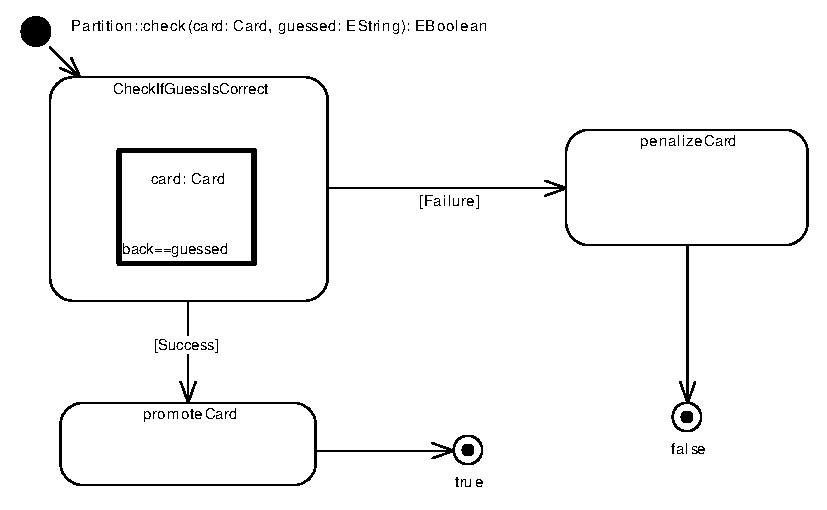
\includegraphics[width=0.8\textwidth]{ea_completeActivityCheck.pdf}
  \caption{Complete SDM for \texttt{Partition::check}}
  \label{fig:sdm_check_finish}
\end{center}
\end{figure}

\item[$\blacktriangleright$] Type in \texttt{true} as the value of the expression (Fig.~\ref{fig:sdm_check_literal_exp}) and complete the SDM by returning
\texttt{false} after penalising a card. Ensure that your SDM (the control flow) closely resembles Fig.~\ref{fig:sdm_check_finish}.

\item[$\blacktriangleright$] As always, export the project, generate code and inspect the implementation for \texttt{check}.  We strongly recommend that you
even write a simple JUnit test (take a look at our simple test case from Part I for inspiration) to take your brand new SDM for a test-spin.


\item[$\blacktriangleright$] Great job - \texttt{check} is now complete! To see how this is implemented in the texual syntax, see Figs.
\ref{fig:completedPatterns} and \ref{fig:finalMethod} in the following section.

\fancyfoot[R]{ $\triangleright$ \hyperlink{sec:emptyPartition}{Next SDM} }

\end{itemize}
